% Chapter 2

\chapter{Background} % Write in your own chapter title
\label{Chapter2}
\lhead{Chapter 2. \emph{Background}} % Write in your own chapter title to set the page header

This work takes heavy use of different techniques, theories and tools mostly 
in the context of compiler construction. To simplify the rest of the thesis 
this chapter explains them as far as necessary, thus I may take
them for granted afterwards. As most of the key ideas will suffice, 
some details will be omitted. 
Interested readers have to fall back on the further readings instead. 


\section{LLVM - The Low Level Virtual Machine}
\label{LLVM}
The Low Level Virtual Machine is a compiler infrastructure designed to optimize
during compiletime, linktime and runtime. Originally designed for C and C++, 
many other frontends for a variety of languages exist by now. The source is 
translated into an intermediate representation (LLVM-IR), which is available 
in three different, but equivalent forms. There is the in-memory compiler IR, 
the on-disk bitcode representation and human readable assembly language.
The LLVM-IR is a type-safe, static single assignment based language,
designed for low-level operations. It is capable of 
representing high-level structures in a flexible way.
Due to the fact that LLVM is built in a modular 
way and can be extended easily, most of the state of the art analysis and
optimization techniques are implemented and shipped with LLVM. Plenty of other
extensions, e.g., Polly, can be added by hand. 


\subsection*{Further Reading}

\begin{itemize}
  \item A Compilation Framework for Lifelong Program Analysis \& Transformation
    \cite{LLVM:CGO04}  
  \item \url{http://www.llvm.org} \nocite{LLVM:Online}
\end{itemize}



\section{The Polyhedral Model}
The polyhedral model is a mathematical way to describe the iteration space of a
subset of all loop nests. Its became popular because it can be used to abstract
from the given source and apply loop optimizations in a pure mathematical way. 

\begin{definition}[Polytope]
  A polytope P in an $n$-dimensional space restricted by $m$ inequalities is defined as:
  \[ \text{P}:= \{ x \in \mathbb{Z}^n \, |\, Ax\leq b \text{ where $A\in\mathbb{Z}^{m*n} $ and $ b\in\mathbb{Z}^{m}$ are constant } \} \]
  \label{def:polytope}
\end{definition}


\begin{wrapfigure}[]{l}{0.4\textwidth}
  %\vspace*{-5mm}
  \includegraphics[width=0.35\textwidth]{Figures/Polytope2d.eps}
  \caption{2-dimensional polytope}
  \label{fig:Polytope2d}
\end{wrapfigure}
Within the polyhedral model the iteration space is modelt as a $\mathbb{Z}$-polytope,
simply spoken a geometric object with flat surfaces existing in a space of 
any general dimension.  
Definition \ref{def:polytope} restrict all (integer) points within the polytope
to be solutions of an affine system of inequalities and figure \ref{fig:Polytope2d} 
shows an example for dimension $n = 2$ and $m = 4$. If the polytope is bounded 
we may speak of convex polytopes instead. For clarification it is worth to say
that some authors e.g., Benabderrahmane et al. \cite{BPCB10} use the term 
polyhedron instead. 


From the compiler writer perspective, the polytope corresponds to the iteration
space of a loop nest, where all loops have affine bounds and steppings.
Each one corresponds to a dimension of the vector space, thus the 
dimension of the polytope is determined by the depth of the loop nest. 
In addition to the points of the iteration space, the polyhedral model is also
capable of representing loop carried dependencies between two iterations. 
Figure \ref{fig:ExampleLoopNest} illustrates this by relating a simple loop 
nest({\footnotesize A}) to its representation within the polyhedral 
model({\footnotesize B}). The main benefit of 
this representation is that transformations can be done in an optimal manner
using an integer linear programming solver which maximizes the loop nest for 
e.g., parallelism. Such transformations within the model are in fact (composed)
affine transformations with the additional advantage that they implicitly apply 
traditional loop optimizations including tiling, skewing, loop interchange and
unrolling. Using the example in listing \ref{lst:ExampleLoopNest} again we may
end up with a loop nest as in listing \ref{lst:ExampleLoopNestTransformed}. 
Data-locality is increased by introducing the two inner most loops which also 
remove the data dependency from the outer most one, thus the whole loope nest
may be executed in parallel now.

\lstset{frame=none}
\begin{figure}[htbp]
  \centering
  \subfloat[Simple loop nest]{%
    \begin{minipage}[c][0.6\width]{%
           0.45\textwidth}
           \centering%
    \lstinputlisting{Primitives/Code/ExampleLoopNest.c}
    \label{lst:ExampleLoopNest}
    \end{minipage}
  } 
  \subfloat[Polyhedral representation for listing \ref{lst:ExampleLoopNest}]{%
    \begin{minipage}[c][0.6\width]{%
           0.45\textwidth}
           \centering%
    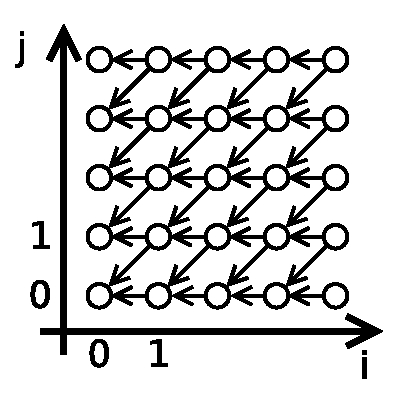
\includegraphics[width=0.55\textwidth]{Figures/ExampleLoopNestPolytope2.eps}
    \label{fig:ExampleLoopNestPolytope}
    \end{minipage}
  }
  
  \subfloat[Optimized version of listing \ref{lst:ExampleLoopNest}]{%
    \lstinputlisting{Primitives/Code/ExampleLoopNestTransformed.c}
    \label{lst:ExampleLoopNestTransformed} 
  }
  \caption{An example loop nest with its polyhedral representation}
  \label{fig:ExampleLoopNest}
\end{figure}
\resetlst



\lstset{frame=none}
\begin{figure}[htbp]
  \centering
\end{figure}
\resetlst

\subsection*{Further Reading}
\begin{itemize}
  \item The Polyhedral Model is More Widely Applicable Than Yoy Think \cite{BPCB10}
  \item Loop Parallelization in the Polytope Model \cite{Lengauer93loopparallelization}  
  \item A practical automatic polyhedral parallelizer and locality optimizer \cite{Bondhugula:2008:PAP:1379022.1375595}
  \item PoCC - The Polyhedral Compiler Collection \cite{PoCC:Online}
  \item Polyhedral parallelization of binary code \cite{Pradelle:2012:PPB:2086696.2086718}
  \item Putting Polyhedral Loop Transformations to Work \cite{BCGST03} 
\end{itemize}

\clearpage

\section{Polly - A Polyhedral Optimizer For LLVM}
\label{Polly}
Exploiting parallelism and data-locality in order to balance the work load
and to improve cache utilization are the main goals of the Polly research project.
The polytope model is used as abstract mathematical representation to get optimal
results for a particular objective. The three-step approach of Polly first detects
maximal loop nests suitable for polyhedral representation. These representations
are analyzed and transformed before they are converted to LLVM-IR again. This 
last step of code generation is capable of generating thread level parallelism 
and vector instructions. The maximal loop nests Polly detects
are called static control parts, or short (valid) SCoPs, are the most central 
entity within Polly and crucial for any kind of argumentation.
%Apart from the
%following descriptions figure \ref{fig:PollyArchitecture} provides an overview
%of the architecture of Polly.



\subsection{Static Control Parts}
\begin{wrapfigure}[]{r}{0.15\textwidth}
  \centering
  %\vspace*{-5mm}
  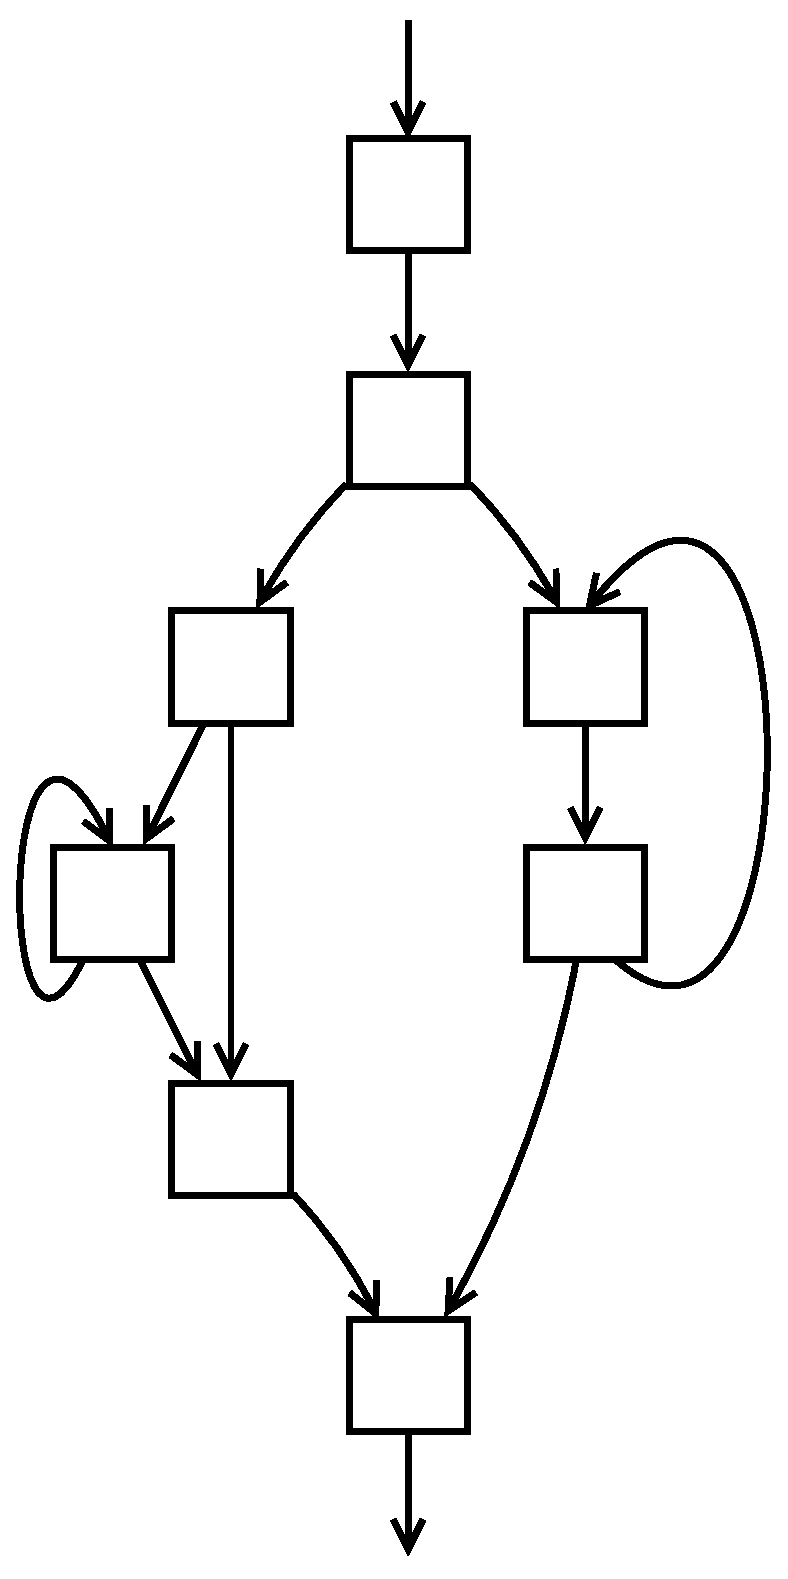
\includegraphics[width=0.15\textwidth]{SimpleRegionCFG.eps}
  \caption{SCoP CFG}
  \label{fig:PossibleSCoPCFG}  
\end{wrapfigure}
A Static Control Part is a subgraph of the control flow graph with one entry
edge and one exit edge. Inside this subgraph only nested conditionals and loops
are allowed (see figure \ref{fig:PossibleSCoPCFG}).
All contained loops need affine bounds and a canonical 
induction variable, thus the lower bound has to be $0$ and the stepping $1$. 
While non affine memory accesses are allowed, all branch conditions have to be
affine functions, only depending on loop invariant parameters and surrounding
induction variables. Aliasing instructions within such a region are not permitted
either. 

While some of these conditions (e.g., the canonical induction variables) 
can be achieved through preprocessing, the rest is still quite restrictive.
Even so, these requirements ensure some very interesting attributes as statically
known control flow and computable memory accesses. The later ones are 
overestimated if a memory access is not affine. If a loop nest fulfills 
these requirements it implicitly has a polyhedral representation which 
can be used for further analyses and transformations. Such regions
are called valid static control parts, or short SCoP. 

SCoPs which do not contain
a loop are not interesting, thus we may consider only SCoPs containing at least
one loop.


%\begin{table}[htbp] 
  %\centering
  %\caption{Restrictions on SCoPs}
    %\begin{itemize}
      %\item Only nested loops and conditionals
      %\item Only branches with affine conditions
      %\item Only affine accesses based on a constant pointer
      %\item No unsigned iteration variables \footnote{}
      %\item No aliasing instructions
      %\item Only canonical PHI nodes and induction variables
      %\item Instructions may not be used in PHI nodes outside the region\footnotemark[1]
      %\item Only ``readnone'' function calls
      %\item No alloca or cast instructions within the region
      %\item Only affine trip counts for loops
      %\item No PHI nodes in the region exit block
      %\item Only simple regions not containing the entry block of the function
      %%\item \textit{A SCoP should contain at least one loop}
    %\end{itemize}
    %\flushleft{\footnotemark[1] open for further work }
  %\label{tab:SCoPConstraints}
%\end{table}



\subsection{SCoP Detection}
Pollys SCoP detection is the gateway to all further analyzses and 
transformations. All regions fulfilling the properties described in the 
last section, or in short, all (valid) SCoPs are detected here. 
The special interest of this part arises from the fact that all 
regions regions declared as valid SCoPs will be considered for pollyhedral 
optimizations. Almost regardless of its content, any region could be given to
Polly if the SCoP detection is instrumented to to so. Two important consequences
can be derived and summarized as:
Utilizing the strenght of Polly is possible in much more situations as 
intentionally implemented but coupled with responsibility of the outcome. 
[TODO ziemlich melodramatisch oder ?]


\subsection{Loop Optimizations}
Polly uses the integer set library (isl) to compute the scheduling and
tiling for a SCoP but it is also possible to use the more matured PoCC optimizer.
Once the polyhedral description is computed, an optimized version of the 
algorithm proposed by Bondhugula et al.\cite{Bondhugula:2008:PAP:1379022.1375595}
will compute a new scheduling and tiling scheme.
Traditional loop
optimizations such as blocking, interchange, splitting, unrolling or unswitching 
are implicitly applied during this step. 
Not only the new scheduling but also the new data dependencies are computed, 
crucial to exploit parallelism.
%Based on these dependencies parallelism is exploited as explained in the next section. 

%\textit{The loop optimizations offers many possibilities in the context 
%of Sambamba (see \ref{FurtherWorkISL}).}


\subsubsection{Parallel Code Generation}
While cache locality is implicitly improved by rescheduling and tiling 
of the loop nest,  parallel code needs to be generated explicitly.
Polly is capable of generating
thread level parallelism using OpenMP annotations and data level parallelism 
using SIMD instructions. The former one depends on the OpenMP shared library 
being present while the later one uses the LLVM built-in vector instruction.


%\begin{figure}[htbp]
  %\centering
  %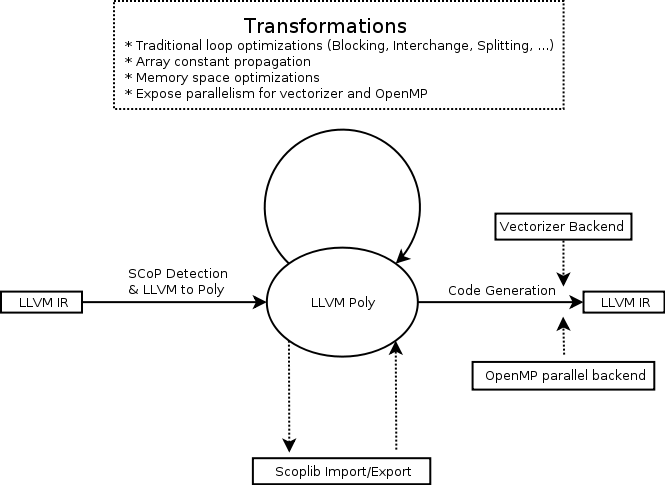
\includegraphics[width=0.9\textwidth]{architecture.png}
  %\caption{Pollys architecture \cite{Polly:Online}}
  %\label{fig:PollyArchitecture}  
%\end{figure}


\subsection*{Further Reading}

\yellow
\begin{itemize}
  \item Polly - Polyhedral optimization in LLVM \cite{grosser.11.impact}  
  \item Enabling Polyhedral Optimizations in LLVM \cite{grosser:thesis}
  \item A Framework for Automatic OpenMP Code Generation \cite{raghesh2011framework}
  \item Base algorithm of isl \cite{Bondhugula:2008:PAP:1379022.1375595}
  \item \url{http://polly.llvm.org} \nocite{Polly:Online}
  \item \url{http://www.kotnet.org/~skimo/isl/} \nocite{ISL:Online}
\end{itemize}





\phantomsection
\section*{2.4 ~ Sambamba \\ A Framework For Adaptive Program Optimization}
\addcontentsline{toc}{section}{2.4 ~ Sambamba - A Framework For Adaptive Program Optimization} 
The Sambamba project is build on top of the LLVM compiler infrastructure and 
aims at adaptive and speculative runtime optimizations.
Dynamic information about arguments or the global state may allow optimization
which could not be applied at compile 
\begin{wrapfigure}[]{r}{0.3\textwidth}
  \centering
  %\vspace*{-5mm}
  \includegraphics[width=0.3\textwidth]{SambambaConcept.eps}
  \caption{Sambamba in a nutshell}
  \label{fig:SambambaConcept}  
\end{wrapfigure}
time or did not seem interesting back then. It is easily extendible with 
compile time and a runtime parts. While each one is conceptually 
independent, the compile time parts may store information which can be accessed
at runtime to reduce the overhead, even if expensive analysis results are needed. 
Another fundamental pillar of the framework is the multi versioning system which
allows for different, specialized function versions. [TODO should VMAD be mentioned here]
A similar approach has
been published by Jimborean et al.\cite{JIMBOREAN-2012-664345}, in fact th
In both cases a dispatcher is used to choose one of the available 
implementations each time the function is called. 
In this manner exclusive optimizations can be applied on the same function and
according to the input a version can be dispatched. Runtime profiling also 
reveals opportunities to speculatively transform the program and obtain more
specialized versions. A main difference between Sambamba and the work of 
Jimborean is probably how these function versions are constructed. Sambamba does
not rely on source code annotations but allows all modules to find and extract
the versions fully automatic. A high level view on the Sambama concept is given
by figure \ref{fig:SambambaConcept} before some of the  built-in utilities 
and modules, used during this work, are explained. 


\clearpage
\subsection{Sambambas Parallelizer}
\begin{wrapfigure}[]{l}{0.45\textwidth}
  \centering
  %\vspace*{-10mm}
  \includegraphics[width=0.43\textwidth]{TransactionQueue.eps}
  \caption{Symboliced transaction queue with 3 worker threads}
  \label{fig:TransactionQueue}  
\end{wrapfigure}
The Sambamba parallelizer will become the main interface for any kind of 
parallelization in the framework. At the moment it is in need of parallel control
flow graphs to explicitly state section which should be executed in parallel, but
in the future more automatic loop parallelization will be implemented too. 
The runtime part of the parallelizer instantiates its own worker threads so there
is no need for external libraries (as OpenMP) in order to execute tasks in parallel. \\


\subsection{Parallel Control Flow Graphs}
\begin{wrapfigure}[]{r}{0.35\textwidth}
  \centering
  \vspace*{-5mm}
  \begin{minipage}[c][0.37\width]{\textwidth}
  \includegraphics[width=0.33\textwidth]{ParallelSectionEx.eps}
  \end{minipage}
  \caption{A parallel section with 3 transactions}
  \label{fig:ParallelSectionEx}  
\end{wrapfigure}
A parallel control flow graph (ParCFG) is a data structure used by the
parallelizer to express parallel sections within an ordinary CFG. 
Each parallel sections consist of an entry block called \texttt{piStart} and
an exit block called \texttt{piEnd}. The \texttt{piStart} is terminated by a 
symbolic switch statement which may have an arbitrary number of predecessors. 
Every predecessor denotes a, so called, transaction which ends in the 
\texttt{piEnd} block after some arbitrary computation. 
Once parallelized each transaction may be executed.
Figure \ref{fig:ParallelSectionEx} shows such a parallel section with 3 
transactions. 


\subsection*{Further Reading}
\begin{itemize}
  \item Sambamba: A Runtime System for Online Adaptive Parallelization \cite{DBLP:conf/cc/StreitHZH12}  
  \item \url{http://www.sambamba.org} \nocite{StreitHZH12:Online}
\end{itemize}



